\resizebox{\textwidth}{!}{%
    \centering
    \scriptsize
    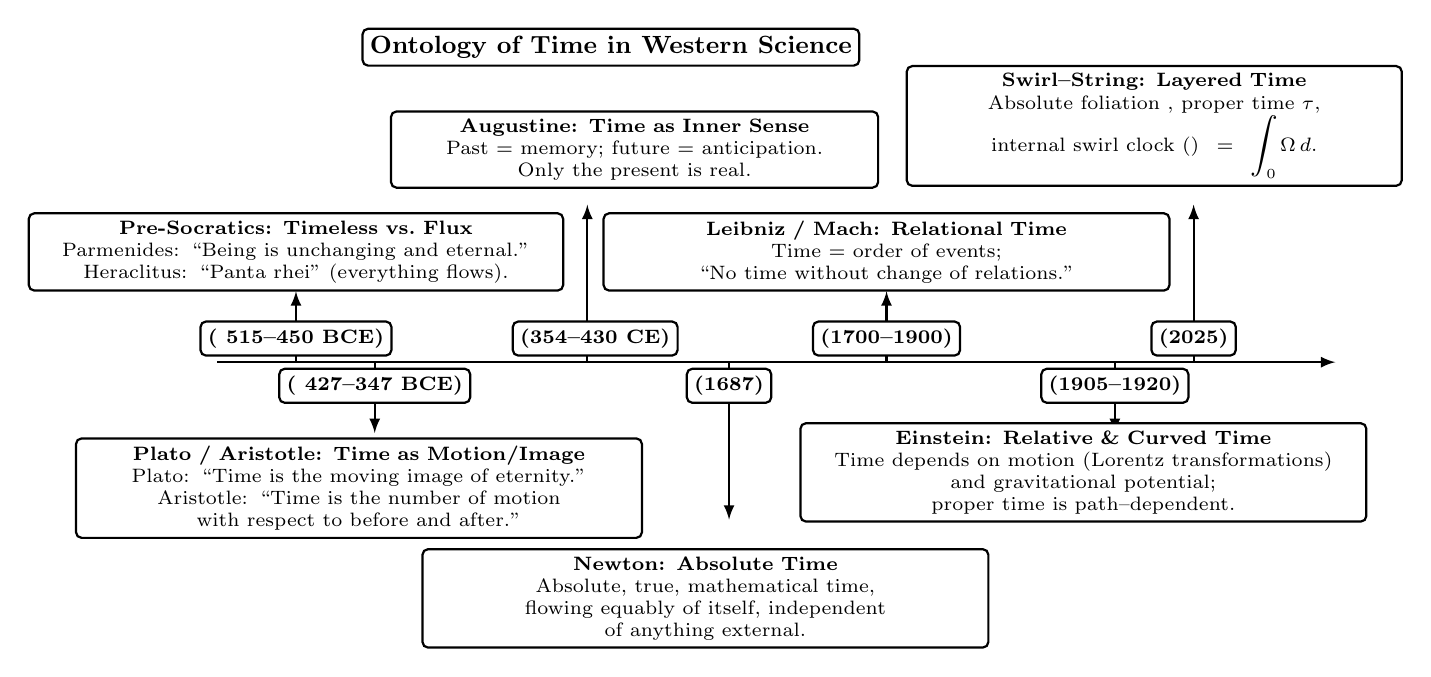
\begin{tikzpicture}[node distance=3.5cm, every node/.style={font=\scriptsize}, >=latex]
        \scriptsize

        % Timeline base
        \draw[->, thick] (-1,0) -- (13.2,0);

        % Arrows above timeline (short)
        \draw[->, thick] (0,0) -- (0,0.9);       % Pre-Socratics
        \draw[->, thick] (3.7,0) -- (3.7,2.0);   % Augustine
        \draw[->, thick] (7.5,0) -- (7.5,0.9);   % Relationalists slot
        \draw[->, thick] (11.4,0) -- (11.4,2.0); % Swirl–String

        % Arrows below timeline (short)
        \draw[->, thick] (1.0,0) -- (1.0,-0.9);     % Plato/Aristotle
        \draw[->, thick] (5.5,0) -- (5.5,-2.0);     % Newton
        \draw[->, thick] (10.4,0) -- (10.4,-0.9);   % Einstein

        %--- Date cards (above timeline) ---
        \node[draw, thick, rounded corners=2pt, fill=white, align=center, font=\bfseries ] at (0, .3)   {(~515--450 BCE)};
        \node[draw, thick, rounded corners=2pt, fill=white, align=center, font=\bfseries ] at (3.8, .3) {(354--430 CE)};
        \node[draw, thick, rounded corners=2pt, fill=white, align=center, font=\bfseries ] at (7.5, .3) {(1700--1900)};
        \node[draw, thick, rounded corners=2pt, fill=white, align=center, font=\bfseries ] at (11.4, .3){(2025)};

        %--- Date cards (below timeline) ---
        \node[draw, thick, rounded corners=2pt, fill=white, align=center, font=\bfseries ] at (1.0,- .3) {(~427--347 BCE)};
        \node[draw, thick, rounded corners=2pt, fill=white, align=center, font=\bfseries ] at (5.5,- .3) {(1687)};
        \node[draw, thick, rounded corners=2pt, fill=white, align=center, font=\bfseries ] at (10.4,- .3) {(1905--1920)};

        % Label
        \node[draw, thick, fill=white, rounded corners=2pt, font=\small] at (4,4.0) {\textbf{Ontology of Time in Western Science}};

        % Pre-Socratics
        \node[draw, rounded corners=2pt, thick, align=center, fill=white, text width=6.6cm] at (0,1.4) {
            \textbf{Pre-Socratics: Timeless vs.\ Flux}\\
            Parmenides: ``Being is unchanging and eternal.''\\
            Heraclitus: ``Panta rhei'' (everything flows).
        };

        % Plato / Aristotle
        \node[draw, rounded corners=2pt, thick, align=center, fill=white, text width=7cm] at (0.8,-1.6) {
            \textbf{Plato / Aristotle: Time as Motion/Image}\\
            Plato: ``Time is the moving image of eternity.''\\
            Aristotle: ``Time is the number of motion\\
            with respect to before and after.''
        };

        % Augustine
        \node[draw, rounded corners=2pt, thick, align=center, fill=white, text width=6cm] at (4.3,2.7) {
            \textbf{Augustine: Time as Inner Sense}\\
            Past = memory; future = anticipation.\\
            Only the present is real.
        };

        % Newton
        \node[draw, rounded corners=2pt, thick, align=center, fill=white, text width=7cm] at (5.2,-3.0) {
            \textbf{Newton: Absolute Time}\\
            Absolute, true, mathematical time,\\
            flowing equably of itself, independent\\
            of anything external.
        };

        % Leibniz / Mach (relational)
        \node[draw, rounded corners=2pt, thick, align=center, fill=white, text width=7cm] at (7.5,1.4) {
            \textbf{Leibniz / Mach: Relational Time}\\
            Time = order of events;\\
            ``No time without change of relations.''
        };

        % Einstein
        \node[draw, rounded corners=2pt, thick, align=center, fill=white, text width=7cm] at (10.0,-1.4) {
            \textbf{Einstein: Relative \& Curved Time}\\
            Time depends on motion (Lorentz transformations)\\
            and gravitational potential; proper time is path--dependent.
        };

        % Swirl–String (modern layered time)
        \node[draw, rounded corners=2pt, thick, align=center, fill=white, text width=6.1cm] at (10.9,3.0) {
            \textbf{Swirl--String: Layered Time}\\
            Absolute foliation \( \Nabs \), proper time \( \tau \),\\
            internal swirl clock \( \Sswirl(\Nabs)=\displaystyle\int_{0}^{\Nabs}\!\Omega\,d\Nabs \).
        };

    \end{tikzpicture}
    \caption{\textbf{Historical progression of time concepts from metaphysics to field theory.} The diagram traces Western ontologies of time—from eternal being and motion--based time, through Newtonian absolutes and Einsteinian relativity, to a swirl--string layered temporal framework: absolute foliation \( \Nabs \), proper time \( \tau \), and internal swirl clock \( \Sswirl \).}
    \label{fig:history-temporal-ontology}
}